\section{Modello di sviluppo}
Il gruppo \emph{Code of Duty} ha scelto di utilizzare il modello incrementale come modello di sviluppo per la produzione del software \hd .
\subsection{Modello incrementale}
Il modello incrementale è un modello di sviluppo di un progetto basato sulla successione dei seguenti passi principali:
\begin{itemize}
	\item Pianificazione;
	\item Analisi dei requisiti;
	\item Progetto;
	\item Implementazione;
	\item Prove;
	\item Valutazione.
\end{itemize}
Il ciclo verrà ripetuto fino a che la valutazione del prodotto diviene soddisfacente rispetto ai requisiti previsti.
L'utilizzo di questo modello è consigliabile in quanto fin dall'inizio della progettazione si ha una visione chiara 
dell'intero progetto in quanto occorre fare in modo che la realizzazione della generica versione K risulti utile per 
la realizzazione della versione K+1.
Il modello di sviluppo incrementale presenta però anche alcuni svantaggi, ad ogni ripetizione del ciclo il codice si complica, 
peggiorando la leggibilità e la manutentabilità rendendo più complicati i successivi incrementi, è comunque possibile porne rimedio tramite refactoring.
Il refactoring o code refactoring è una tecnica strutturata per modificare la struttura interna di porzioni di codice senza modificarne
il comportamento esterno, viene utilizzata per migliorare alcune caratteristiche non funzionali del software quali la leggibilità e la manutenibilità e la riusabilità del codice.
\begin{figure}[H]
        \centering
        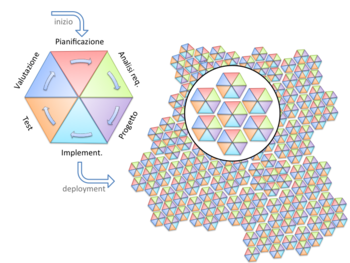
\includegraphics[width=0.5\textwidth]{source/img/modelloincrementale.png}
        \caption{Rappresentazione grafica del Modello Incrementale}
\end{figure}
